\chapter{Metodologia di Sviluppo}

\begin{figure}[!hbt]
  \centering
  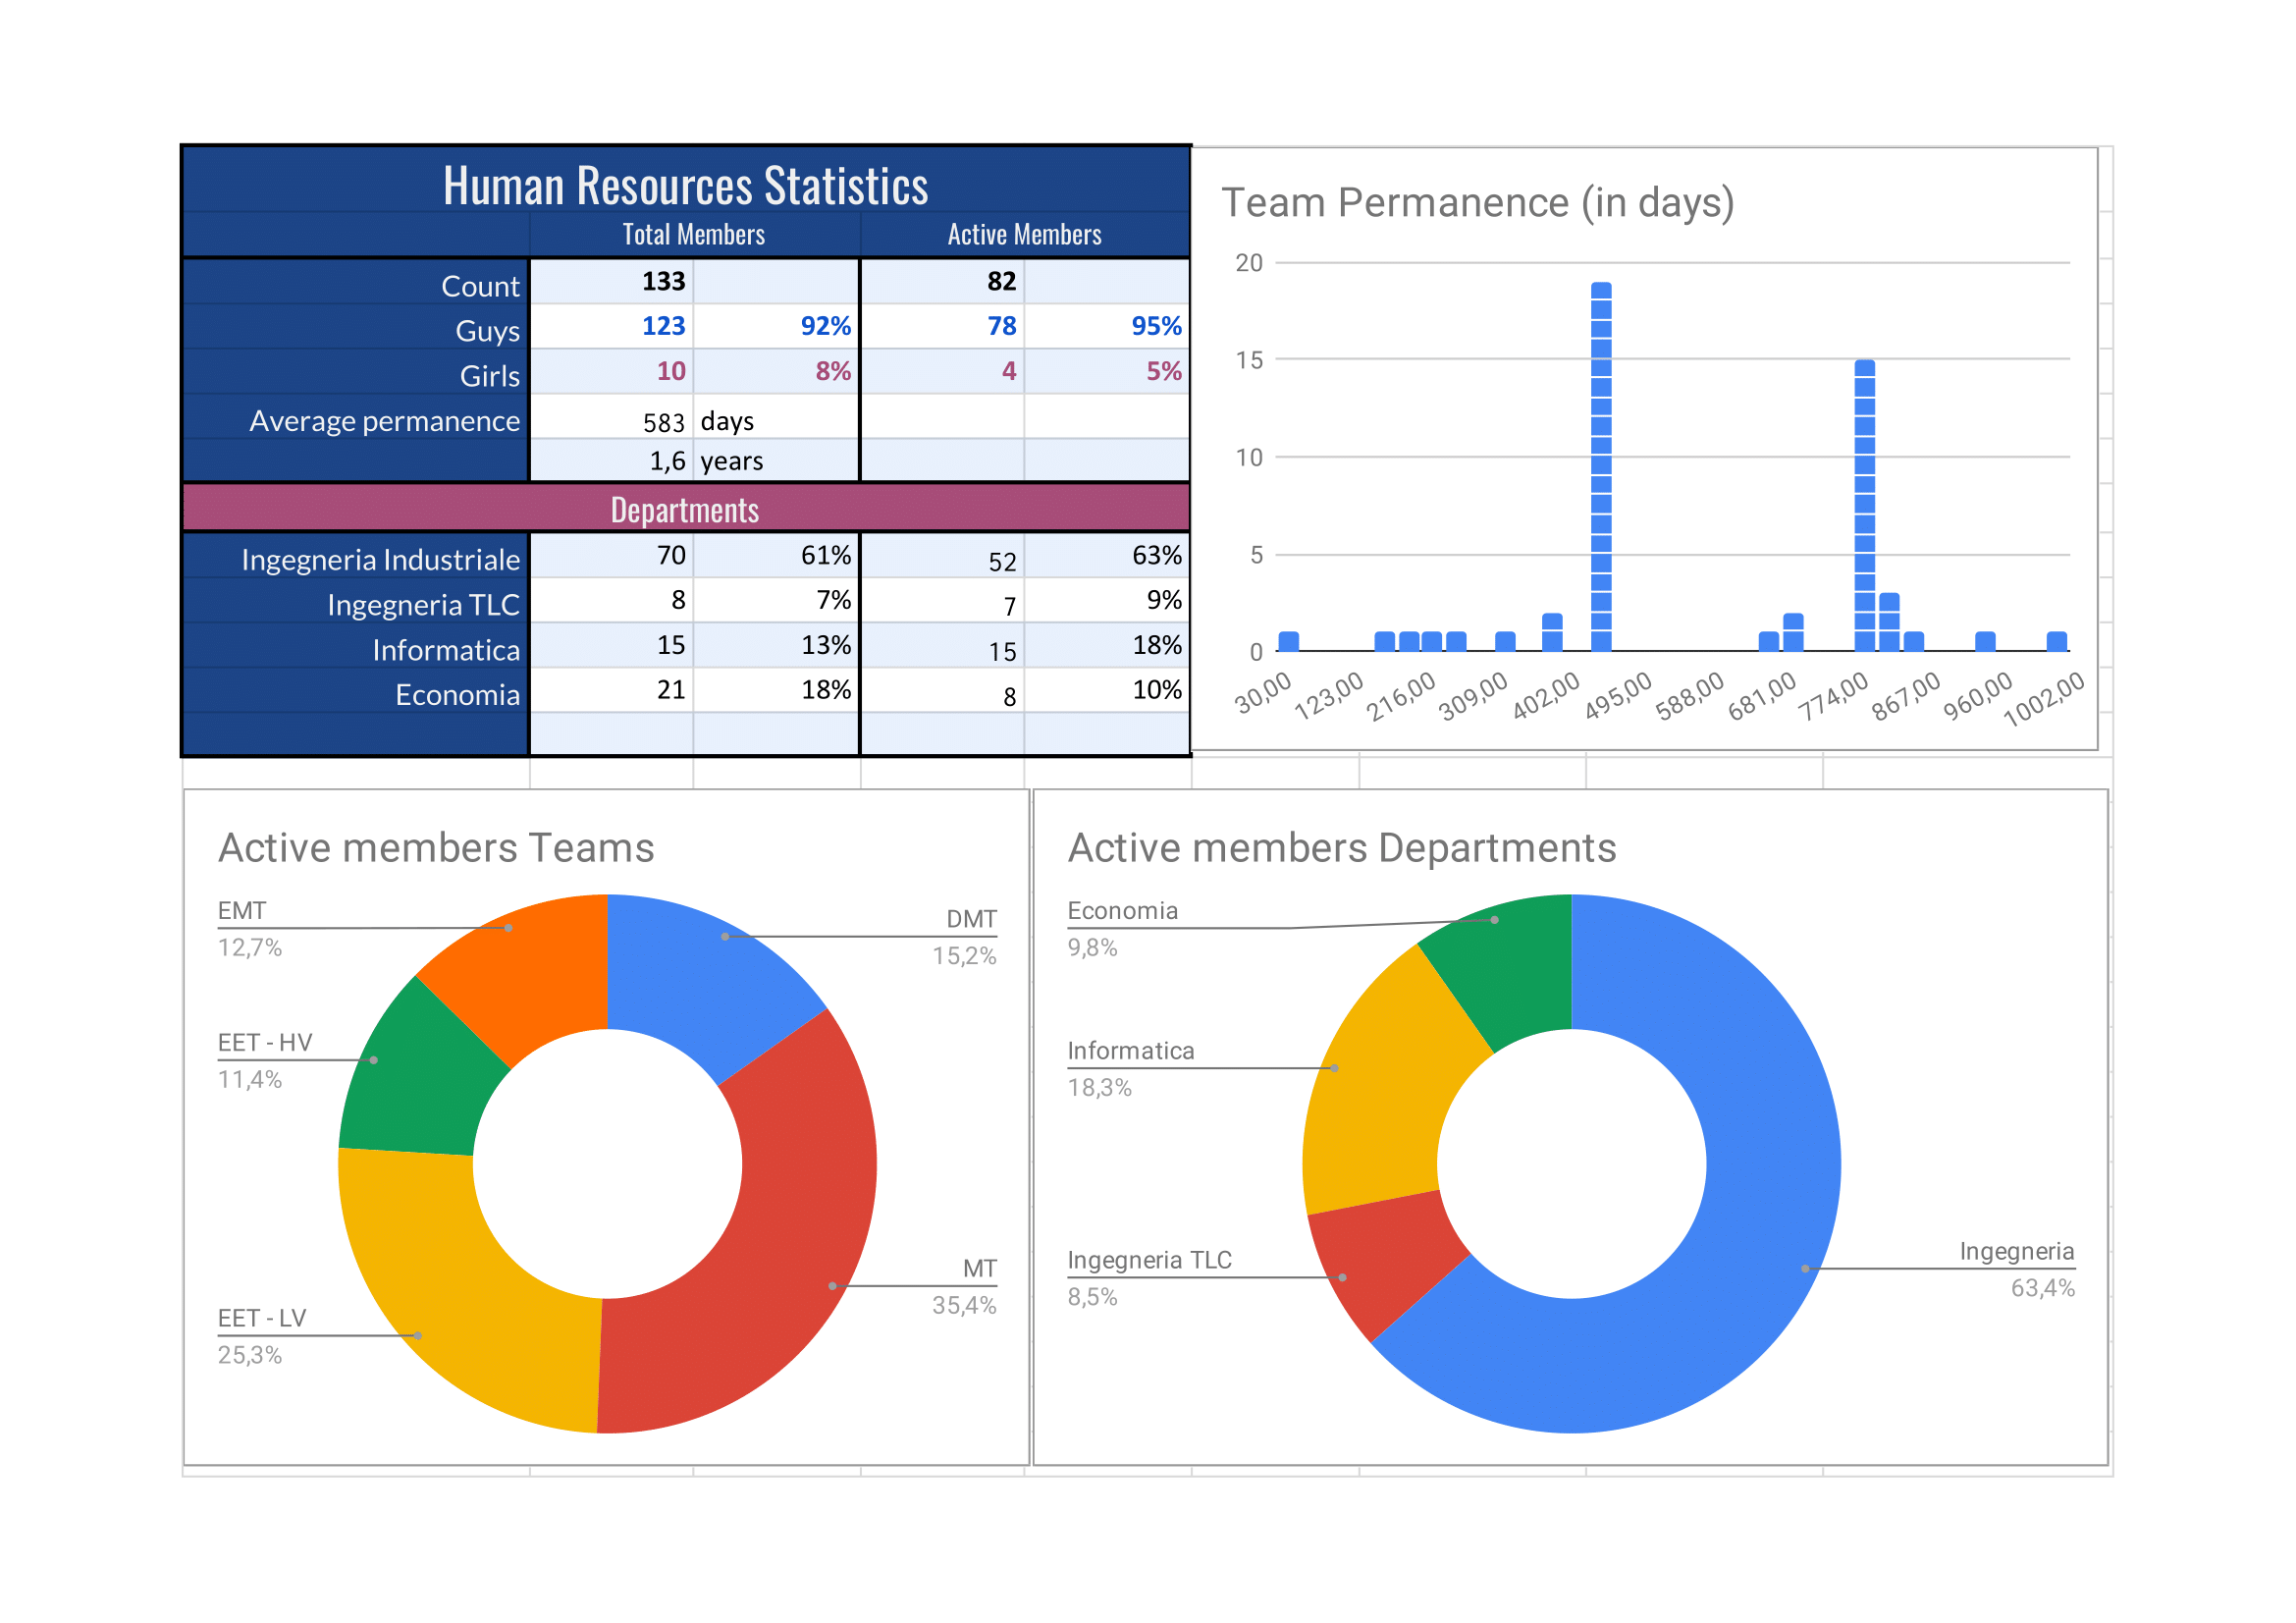
\includegraphics[width=0.75\textwidth]{./figures/membri.png}
  \caption{E-Agle Trento Racing Team}
\end{figure}

L'organizzazione del Team a Settembre 2017 dal punto di vista software non era ben definita, 
alcune parti di codice erano presenti online, altre solo mantenute in locale dalle persone interessate.
Questa modalità ha avuto molti limiti, soprattutto per quanto riguarda il version controlling e l'aggiornabilità del codice, 
non avendo la possibilità di mantenere diverse versioni in paralello.
Per cui confrontadoci con gli altri studenti si è deciso di avere un profilo pubblico della squadra su GitHub per poter mantenere il codice
secondo gli standard attuali e poterlo condividere con chi d'interesse. La scelta di GitHub è stata spontanea, dovuta ai suoi vantaggi rispetto
a BitBucket per la partnership con l'unversità e quindi tool inclusi.
Questo ha migliorato notevolmente il workflow di chi lavorava sulle varie parti della macchina e il tempo di apprendimento degli studenti che hanno deciso di avvicinarsi al progetto
soprattuto grazie alla realizzazione, attraverso Sphinx e GitHub Pages, di una raccolta di documentazioni e procedure da tramandare. 

\newpage

\section{GitHub e Documentazione}

I due principali strumenti introdotti sono stati GitHub per il version controlling e 
la condivisone del codice e Sphinx per generare documentazione partendo da documentazioni che altri studenti avevano già scritto.

L'approccio a GitHub è stato lento, ma ha permesso di poter dare uno spazio a tutto il codice del Team in breve tempo.
Le repository sono gestite da un admin che si occupa di aggiungere gli studenti interessati e consiglia come mantenere il codice grazie a controlli periodici.
La struttura delle repository è definita in base alla monoposto e al sottogruppo di interesse, o più in generale una parte della macchina. 
Un esempio sono le due versioni del Volante, \emph{chimera-steeringwheel} \cite{chimera-telemetria} e \emph{fenice-steeringwheel} \cite{fenice-steeringwheel}.
Per quanto riguarda la repository del Volante è stato deciso di mantenerla pubblica.
Essendo un progetto universitario che vede l'impegno di più persone sotto più ambienti (software, hardware e meccanico)
ci è sembrata la scelta giusta presentare l'esempio di una interfaccia unica nel suo genere che utilizza diverse tecnologie
da cui le persone possono ispirarsi e utilizzarla come esempio per le librerie del framework e le tecnologie usate.

L'introduzione di Sphinx è nata dalla necessità di condividere le conoscenze con altri studenti che si avvicinano al progetto 
e trovare un punto raccolta unico e accessibile da esterni del materiale ritenuto utile e non sensibile.
La scelta di utilizzare Sphinx come strumento è dovuta alla consultazione, in quel periodo, di alcune documentazioni relative a schede
programmabili con Python. Questa documentazione mi è sembrata fin da subito semplice e facilmente mantenibile da parte di tutti.
Una delle prime guide pubblicate è stata \emph{"Come cross-compilare per Raspberry da Linux"} per il framework Qt, 
siamo partiti da una guida trovata su Medium \cite{Medium} per arrivare alla nostra versione per il Team Telemetria.
La scelta di utilizzare Sphinx come generatore di documentazione ha mostrato un grande vantaggio quando è stato deciso di rendere pubblico 
il materiale della Design Presentation. 

\begin{figure}[!hbt]
  \centering
  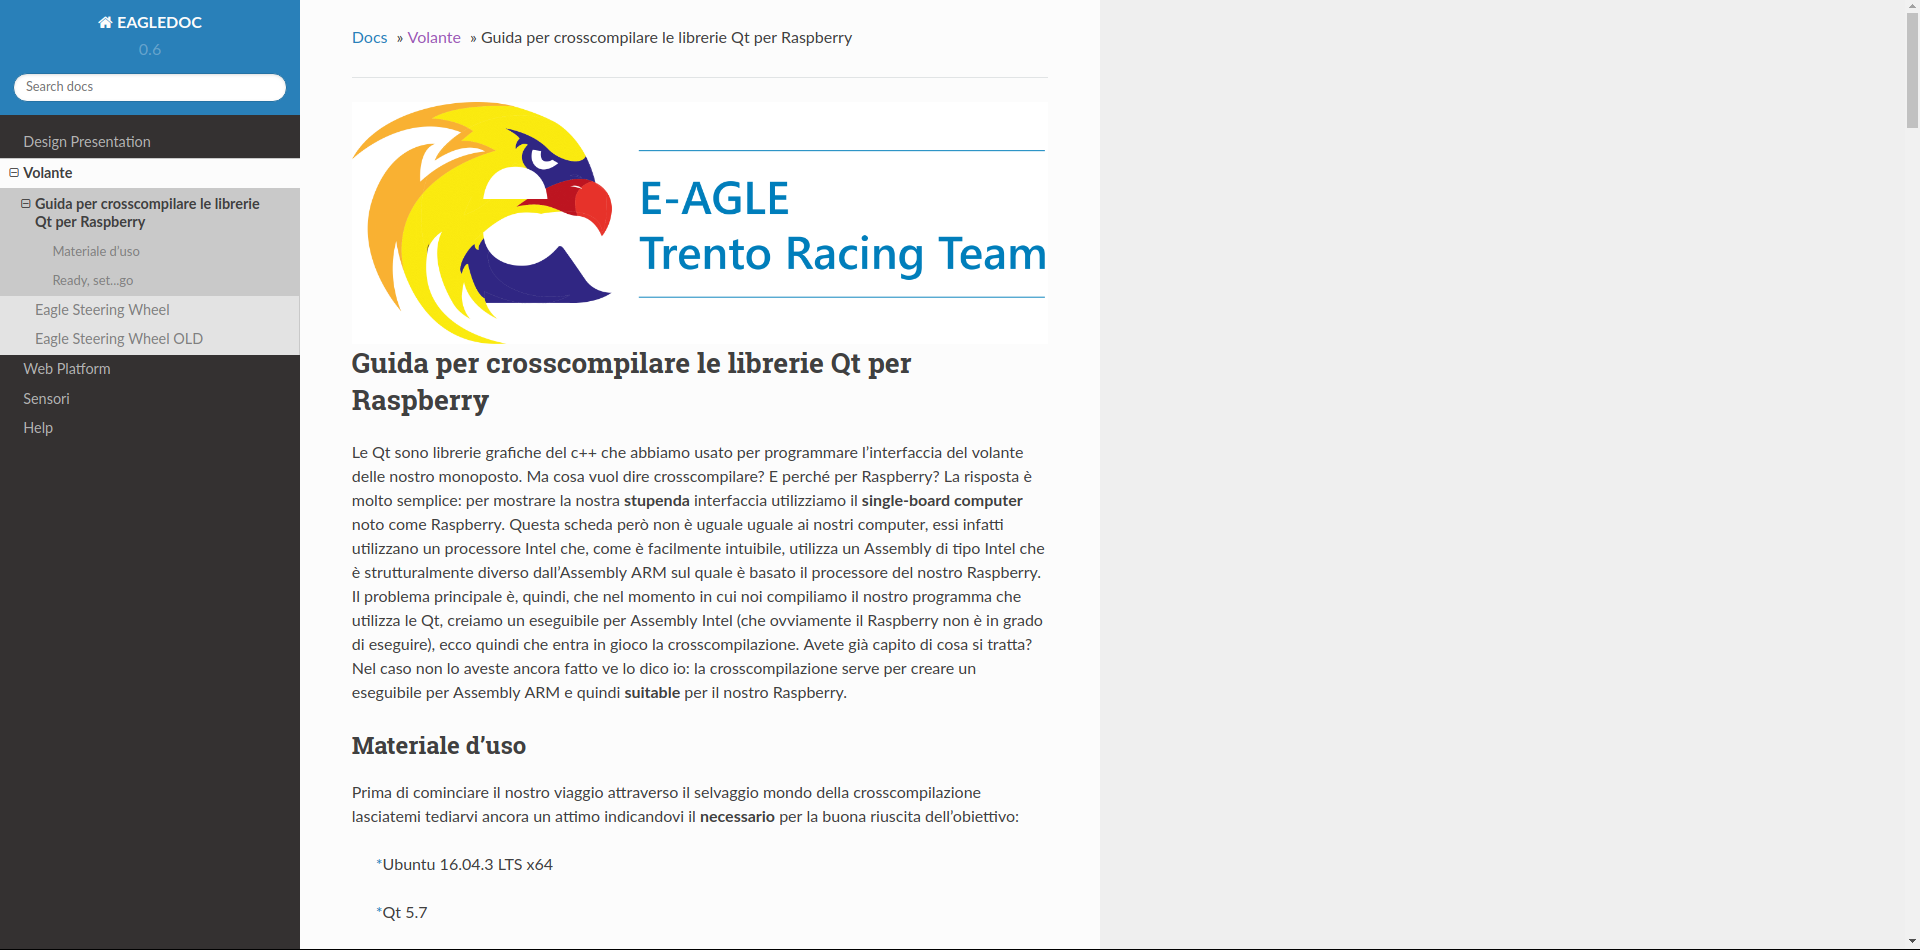
\includegraphics[width=0.75\textwidth]{./figures/sphinx.png}
  \caption{Sito Documentazione del Team \cite{eagletrt.github.io}}
\end{figure}

Questi materiali sono stati portati dal formato \emph{.docx} a \emph{.rst}, utilizzato da Python per creare pagine \emph{.html} statiche.
Sono state poi rese disponibili online e accessibili attraverso QR code dai nostri rollup che esponiamo durante gli eventi.
Il risultato è stato quello di poter mostrare agli sponsor e alle persone interessate al progetto il lavoro svolto per ogni componente realizzata da noi
e le scelte tecniche fatte.

\newpage

\section{Organizzazione Team e Attività}

% Sviluppo agile perchè ci è sembrata la più adatta
% Tavole Kanban per tutti grazie a waffle.io
% Divisione Team 

Durante le riunioni con il gruppo telemetria ho riscontrato delle difficoltà da parte dei membri
nell'organizzazione del lavoro e nell'avere chiari gli step necessari per il raggiungemento dell'obbiettivo principale.
Per ovviare a questo problema si è rivelato molto utile un approccio \emph{agile} e l'utilizzo di tavole \emph{kanban}.

Predisporre il team all'utilizzo di metodi agili ci ha permesso di ridurre il rischio di fallimento 
durante lo sviluppo, testando in locale e poi portando in macchina la funzionalità senza riscontrare errori.
Il problema principale che emerge dai partecipanti al progetto è quello di non poter dedicare
il tempo che desiderano al team, avere un approcio \emph{agile} ci ha permesso di sviluppare in breve tempo e in modo 
ordinato tutto quello che ci veniva richiesto venendo incontro alle esigenze dei singoli.

Il risultato è stato un approccio diviso in queste fasi:
 
\begin{itemize}
  \item Pianificazione: Determinare, concordando con i membri del team attraverso riunioni e/o resoconti dei test, quale funzionalità deve essere implementata.
  \item Analisi dei requisiti: Come può essere integrata la funzionalità all'interno del nostro codice, valutando librerie e tecniche alternative.  
  \item Progettazione: Divisa in due parti, la prima, molto importante nel nostro caso, disegno su carta per poi passare alla seconda che riguarda la stesura del codice. 
  \item Test: Svolti principalmente in locale e poi portati sul dispositvo senza riscontrare problemi di compatibilità.
\end{itemize}

Per quanto riguarda il Volante inteso come \emph{"prodotto finito"} i passi necessari sono stati più articolati.
Tutti i membri del gruppo si sono occupati di raccogliere delle possibili soluzioni per poi essere discusse e
confrontate anche con chi non era coinvolto direttamente, per poter condvidere il più possibile il \emph{know-how}.
Attraverso riunioni periodiche e la raccolta di feedback sulla nostra monoposto è stato possile, grazie alla disponibilità
delle persone coinvolte, di avere sempre chiaro cosa andava e cosa no. 
Questo è stato molto importante perchè ha definito una tipologia di task specifica che ogni membro del team, non per forza 
coinvolto nello sviluppo software, doveva portare a termine.

\begin{figure}[!hbt]
  \centering
  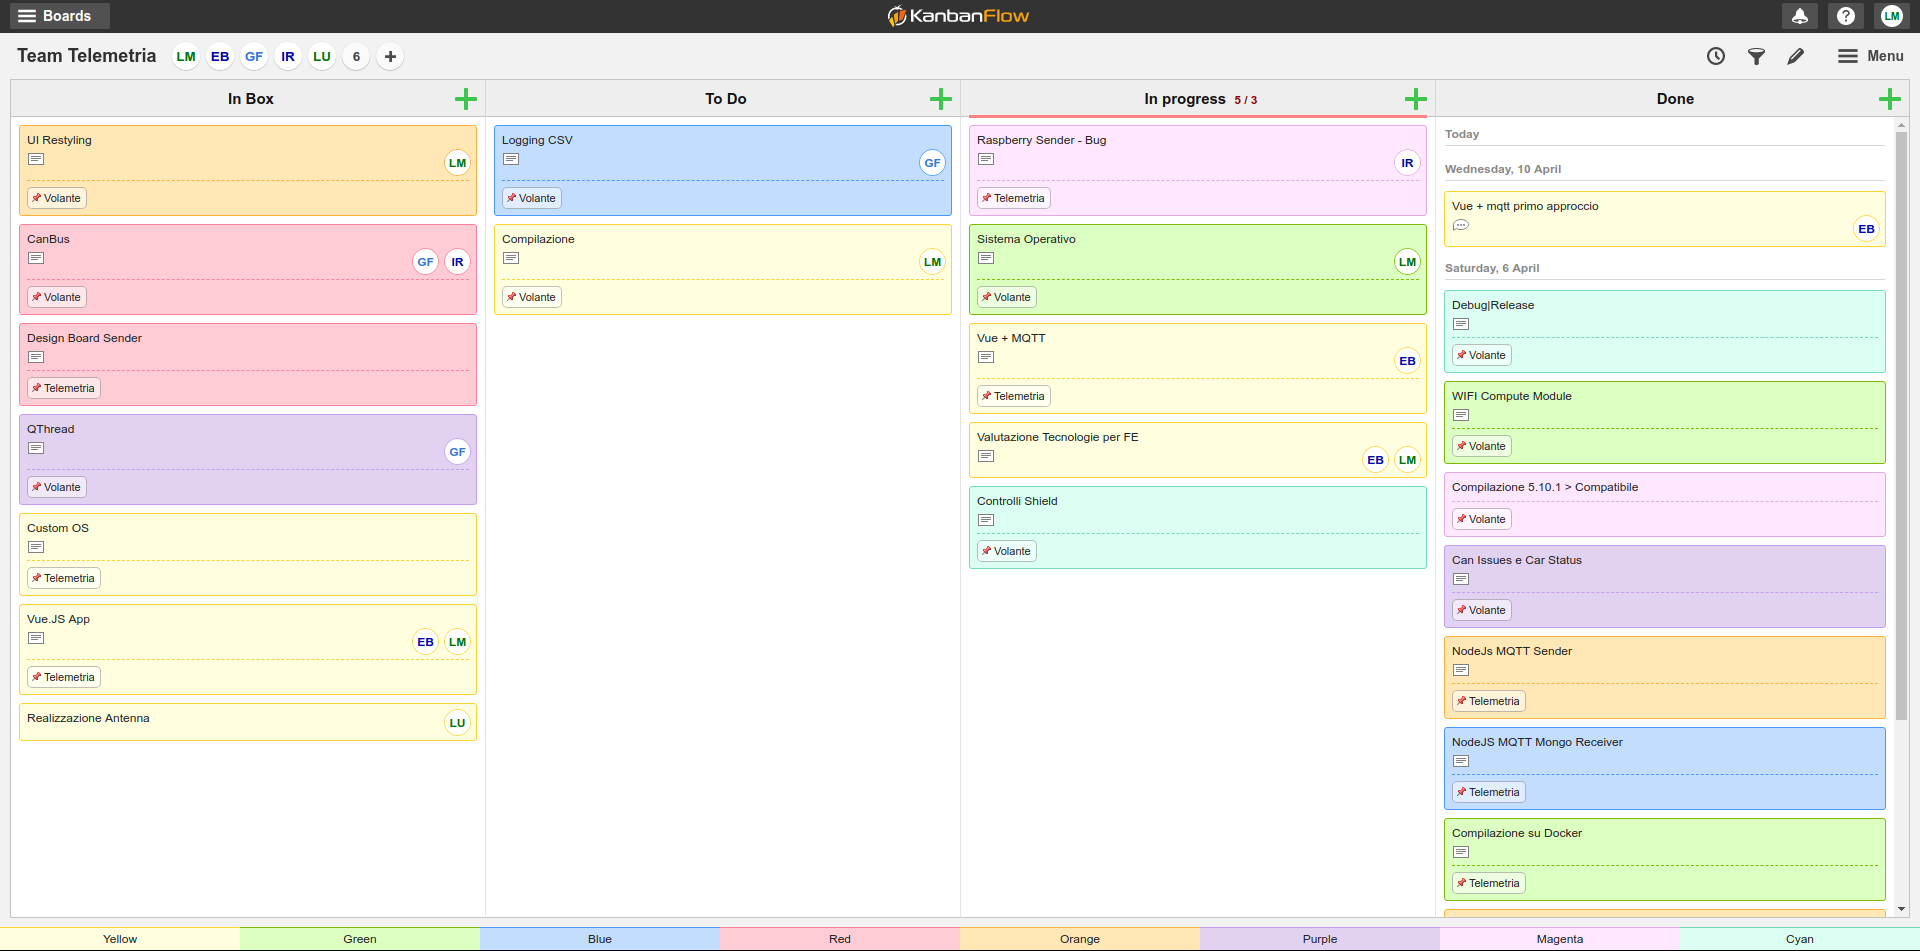
\includegraphics[width=0.75\textwidth]{./figures/kanban.png}
  \caption{Tavola Kanban utilizzata dal Team Telemetria}
\end{figure}

L'introduzione di Kanban ha migliorato il flusso di lavoro, aumentato la produttività e la qualità del prodotto finale in modo considerevole. 
Kanban fa parte dei metodi agili e come tale rende il processo lavorativo molto più flessibile, 
non sempre le task sono state portate a termine nelle scadenze prestabilite, 
questo per impegni universitari e mancanza di esperienza nello stimare i tempi. 
I compiti sono stati suddivisi in piccole task e portati a termine l’uno dopo l’altro. 
Tuttavia data la sua flessibilità abbiamo sempre mantenuto indipendete lo sviluppo di una parte rispetto ad un'altra e grazie alla facilità 
di creare prototipi in grado di testare le singole funzionalità in poco tempo non si sono mai trovate delle situazioni in cui non potevamo testare 
perchè non avevamo un finito una task. 
Lo sviluppo in parallelo, considerato come attività multitasking, è stato sempre mantenuto in quanto le competenze dei singoli membri del team erano sempre 
abbastanza specifiche. 

Il team che si è occupato dello sviluppo del Volante e della sua realizzazione è composto da:
\begin{itemize}
  \item Davide Farina: Pilota e supervisore del progetto
  \item Luca Martinelli: Main Developer
  \item Daniele Faccinelli: PCB Designer 
  \item Laura Scoccianti: UI Designer
  \item Ciro Malacarne: Case Designer
  \item Damiano Iob: Responsabile del Sistema Operativo
\end{itemize}

Ogni parte dello sviluppo è stata messa su Gantt e poi, per avere una visione specifica del lavoro, 
le fasi del Gantt sono state espanse e analizzate come tante singole task identifiacando poi la fine come una \emph{Milestone}.
Nel 2019 come strumento è stato utilizzato \emph{waffle.io}, in quanto è facilmente integrabile con la repository GitHub.
Quest'anno, invece, causa la chiusura del sito, ci siamo spostati a \emph{Kanban Flow} perchè non avendo esigenze particolari qualsiasi applicazione web
poteva fare al caso nostro. L'unico requisito è stato la semplicità d'uso e avere più progetti nello stesso tempo.
Gli studenti coinvolti, anche se non direttamente interessati allo sviluppo software, utilizzavano la tavola kanban per avere sempre sotto 
mano lo stato dei lavori. Per quanto riguarda la creazione di nuove task, e più in generale, la sua gestione, se ne è occupato l'amministratore. 

% conseguenze? scelte tecniche (e) specifiche vincenti grazie al confronto di persone diverse con lo stesso scopo

Una considerazione importante da fare è che questi problemi sono emersi durante la mia presenza nel team e precedentemente non erano mai stati rilevati.
Lo scopo principale fin da subito è stato la realizzazione della macchina e mentre c'è stata attenzione per l'organizzazione in senso 
generale si è trascurato l'aspetto organizzativo del singolo sotto-team e in particolare dello sviluppo software. 
Le motivazioni sono da trovare nel breve tempo che si ha a disposizone per sviluppare e testare e nell'inesperienza delle persone coinvolte
visto che il progetto è nato da poco e dobbiamo confrontarci con studenti di facoltà 
che hanno squadre con esperienza di oltre 10 anni di competizione.  
L'introduzione di queste tecnologie e la formazione delle persone per approcciarsi ad ess,e ha fatto si che le scelte tecniche potessero essere
prese con più consapevolezza, alle volte in modo indipedente, grazie alla divisione dei compiti in base alle aree di competenza. 
Scelte che si sono poi rivelate vincenti nel corso del progetto.

\newpage

% Durante la sessione invernale, quando decisi che avremmo dovuto ridisegnare l'interfaccia, stavo seguendo il corso di ingegneria del software 2 e sostenendo l'esame di ingegneria del software 1, questo mi ha permesso di mettere in pratica le nozioni teoriche apprese a lezione.
% Questa è stata un parte molto importnate per lo sviluppo di un progetto così vasto in termini di conoscenze di settori specifici, avere chiaro fin da subito il ruolo di ognuno nel team è stato di grande aiuto. 
% Oltre ad averci permesso di ridurre di molto i tempi di sviluppo e test, ci ha dato la possibilità di essere apprezzati da specilisti nel settore non solo per il prodotto ma anche per come sono state affrontate e prese le scelte.

% Il nostro obbiettivo è stato sin da subito fare qualcosa di unico e che altre squadre e case automobilistiche avrebbero potuto vedere, da qui l'esigenza di rendere il codice pubblico  
